\documentclass[a4paper,11pt]{article}
\usepackage[process=auto,cleanup={.tex, .dvi, .pdf, .log}]{pstool}
\usepackage[T2A]{fontenc}
\usepackage[utf8]{inputenc}
\usepackage[english,russian]{babel}
\usepackage{amssymb,amsmath}
\usepackage{gensymb,textcomp,latexsym}
\usepackage{graphicx}
\usepackage{tabularx}
\usepackage[pdftex, left=1in, right=1in, top=1in, bottom=2cm]{geometry}
\usepackage{parcolumns}
\usepackage{multirow}
\usepackage{tikz}
\pagenumbering{gobble}

\newcommand{\figref}[1]{Рис.~\ref{#1}}
\usepackage{epstopdf}
\usepackage{float}

\begin{document}

%\begin{figure}[h]
%	\centering
%	\begin{minipage}{0.49\linewidth}
%		\centering а)\\
%		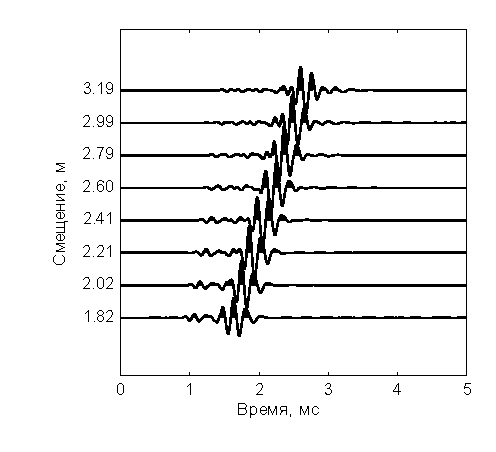
\includegraphics[width=1\linewidth]{./images/nonorth_alford/el15x10_BS_HTI_45_Drot1-pstool.eps} 
%		%\psfragfig[width=0.49\linewidth,crop=pdfcrop]{./images/nonorth_alford/el15x10_BS_HTI_45_Drot1} 	
%	\end{minipage}
%	\begin{minipage}{0.49\linewidth}
%		\centering 
%		б)\\
%		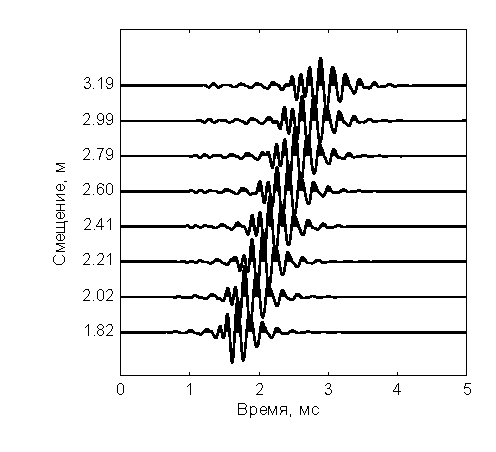
\includegraphics[width=1\linewidth]{./images/nonorth_alford/el15x10_CS_HTI_45_Drot1-pstool.eps}
%		%\psfragfig[width=0.49\linewidth,crop=pdfcrop]{./images/nonorth_alford/el15x10_CS_HTI_45_Drot1}		
%	\end{minipage}
%	\begin{minipage}{0.49\linewidth}
%		\centering 
%		в)\\
%		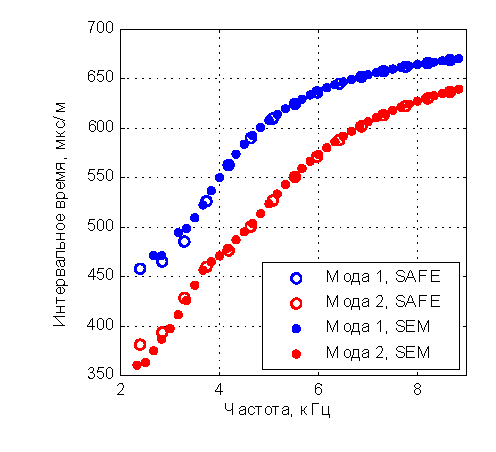
\includegraphics[width=1\linewidth]{./images/nonorth_alford/el15x10_HTI_BS_f45_disp_modes_SAFE-pstool.eps}
%		%\psfragfig[width=0.49\linewidth,crop=pdfcrop]{./images/nonorth_alford/el15x10_HTI_BS_f45_disp_modes+SAFE} 
%	\end{minipage}
%	\begin{minipage}{0.49\linewidth}
%		\centering 
%		г)\\
%		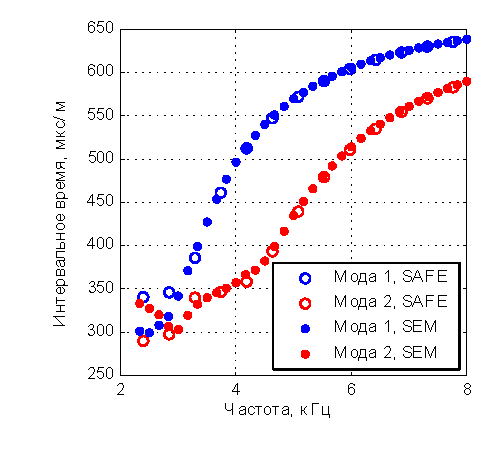
\includegraphics[width=1\linewidth]{./images/nonorth_alford/el15x10_HTI_CS_f45_disp_modes_SAFE_new-pstool.eps}
%		%\psfragfig[width=0.49\linewidth,crop=pdfcrop]{./images/nonorth_alford/el15x10_HTI_CS_f45_disp_modes+SAFE_new} 		
%	\end{minipage}
%	%\caption{\footnotesize Исходные сигнатуры давления для измерения ХХ, смоделированные в SEM, а также дисперсионные кривые для двух дипольных мод в эллиптических скважинах ($15 \times 10$ см) в породах Bakken Shale (а,в) и Cotton Valey Shale (б,г). Дисперсионные кривые на графиках независимо получены модифицированным методом Прони (на основе данных моделирования SEM) и методом SAFE. }
%	%\label{fig:disp_curves_all}
%\end{figure}

\begin{figure}[h]
\centering
{а)} \\
\renewcommand{\arraystretch}{1.5}
\begin{tabular*}{1\textwidth}{c|cc|cc|}
\cline{2-5}
&\multicolumn{2}{c|}{\textbf{Bakken Shale} (12,70$\times$10,16 см)} &\multicolumn{2}{c|}{\textbf{Bakken Shale} (15,00$\times$10,00 см)}\\ 
\begin{minipage}{0.02\textwidth}
\rotatebox{90}{\footnotesize \textit{Дипольная мода 1}} 
\end{minipage}&
\begin{minipage}{0.22\textwidth}
	%\psfragfig[width=0.23\textwidth,crop=pdfcrop]{./images/SAFE/SAFE_BS_10x8_HTI_45/P_s_3_3kHz}	
	
\includegraphics[width=1\linewidth]{./images/SAFE/SAFE_BS_10x8_HTI_45/P_s_3_3kHz-pstool.eps}	
\end{minipage}&
\begin{minipage}{0.22\textwidth}
	%\psfragfig[width=0.23\textwidth,crop=pdfcrop]{./images/SAFE/SAFE_BS_10x8_HTI_45/P_s_5_5kHz}	
	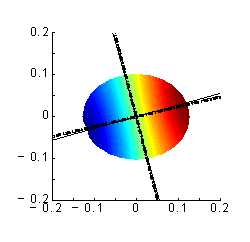
\includegraphics[width=1\linewidth]{./images/SAFE/SAFE_BS_10x8_HTI_45/P_s_5_5kHz-pstool.eps}	
\end{minipage}&
\begin{minipage}{0.22\textwidth}
	%\psfragfig[width=0.23\textwidth,crop=pdfcrop]{./images/SAFE/SAFE_BS_15x10_HTI_45/P_s_3_3kHz}
	
\includegraphics[width=1\linewidth]{./images/SAFE/SAFE_BS_15x10_HTI_45/P_s_3_3kHz-pstool.eps}	
\end{minipage}&
\begin{minipage}{0.22\textwidth}
	%\psfragfig[width=0.23\textwidth,crop=pdfcrop]{./images/SAFE/SAFE_BS_15x10_HTI_45/P_s_5_5kHz}
	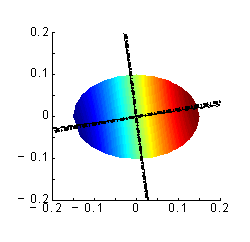
\includegraphics[width=1\linewidth]{./images/SAFE/SAFE_BS_15x10_HTI_45/P_s_5_5kHz-pstool.eps}		
\end{minipage}\\ 
%& & & & \\
\begin{minipage}{0.02\textwidth}
\rotatebox{90}{\footnotesize \textit{Дипольная мода 2}} 
\end{minipage} &
\begin{minipage}{0.22\textwidth}
	%\psfragfig[width=0.23\textwidth,crop=pdfcrop]{./images/SAFE/SAFE_BS_10x8_HTI_45/P_a_3_3kHz}
	
\includegraphics[width=1\linewidth]{./images/SAFE/SAFE_BS_10x8_HTI_45/P_a_3_3kHz-pstool.eps}		
\end{minipage} &
\begin{minipage}{0.22\textwidth}
	%\psfragfig[width=0.23\textwidth,crop=pdfcrop]{./images/SAFE/SAFE_BS_10x8_HTI_45/P_a_5_5kHz}	
	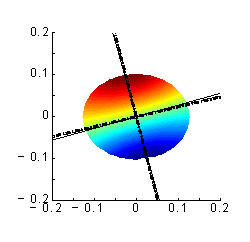
\includegraphics[width=1\linewidth]{./images/SAFE/SAFE_BS_10x8_HTI_45/P_a_5_5kHz-pstool.eps}	
\end{minipage} &
\begin{minipage}{0.22\textwidth}
	%\psfragfig[width=0.23\textwidth,crop=pdfcrop]{./images/SAFE/SAFE_BS_15x10_HTI_45/P_a_3_3kHz}
	
\includegraphics[width=1\linewidth]{./images/SAFE/SAFE_BS_15x10_HTI_45/P_a_3_3kHz-pstool.eps}		
\end{minipage} &
\begin{minipage}{0.22\textwidth}
	%\psfragfig[width=0.23\textwidth,crop=pdfcrop]{./images/SAFE/SAFE_BS_15x10_HTI_45/P_a_5_5kHz}
	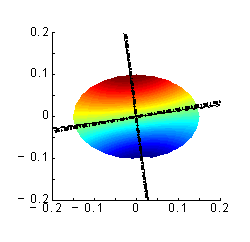
\includegraphics[width=1\linewidth]{./images/SAFE/SAFE_BS_15x10_HTI_45/P_a_5_5kHz-pstool.eps}		
\end{minipage} \\ 
& \footnotesize НЧФ, 3,29 кГц & \footnotesize ВЧФ, 5,53 кГц & \footnotesize НЧФ, 3,29 кГц & \footnotesize ВЧФ, 5,53 кГц \\ \cline{2-5}
\end{tabular*} \\
\quad \\
{б)} \\
\begin{tabular*}{1\textwidth}{c|cc|cc|}
\cline{2-5}
&\multicolumn{2}{c|}{\textbf{Cotton Valey Shale} (12,70$\times$10,16 см)} &\multicolumn{2}{c|}{\textbf{Cotton Valey Shale} (15,00$\times$10,00 см)}\\
\begin{minipage}{0.02\linewidth}
	\rotatebox{90}{\footnotesize\textit{Дипольная мода 1}} 
\end{minipage}&
\begin{minipage}{0.22\linewidth}
	%\psfragfig[width=0.22\linewidth,crop=pdfcrop]{./images/SAFE/SAFE_CS_10x8_HTI_45/P_s_3_0kHz}	
	
\includegraphics[width=1\linewidth]{./images/SAFE/SAFE_CS_10x8_HTI_45/P_s_3_0kHz-pstool.eps}		
\end{minipage}&
\begin{minipage}{0.22\linewidth}
	%\psfragfig[width=0.22\linewidth,crop=pdfcrop]{./images/SAFE/SAFE_CS_10x8_HTI_45/P_s_7_2kHz}	
	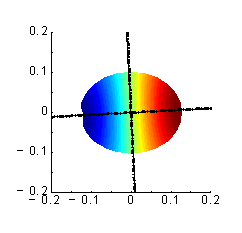
\includegraphics[width=1\linewidth]{./images/SAFE/SAFE_CS_10x8_HTI_45/P_s_7_2kHz-pstool.eps}	
\end{minipage}&
\begin{minipage}{0.22\linewidth}
	%\psfragfig[width=0.22\linewidth,crop=pdfcrop]{./images/SAFE/SAFE_CS_15x10_HTI_45/P_s_3_0kHz}
	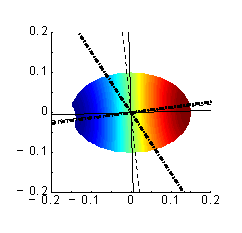
\includegraphics[width=1\linewidth]{./images/SAFE/SAFE_CS_15x10_HTI_45/P_s_3_0kHz-pstool.eps}		
\end{minipage}&
\begin{minipage}{0.22\linewidth}
	%\psfragfig[width=0.22\linewidth,crop=pdfcrop]{./images/SAFE/SAFE_CS_15x10_HTI_45/P_s_7_2kHz}
	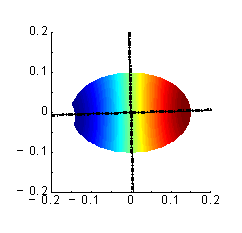
\includegraphics[width=1\linewidth]{./images/SAFE/SAFE_CS_15x10_HTI_45/P_s_7_2kHz-pstool.eps}		
\end{minipage} \\
\begin{minipage}{0.02\linewidth}
	\rotatebox{90}{\footnotesize\textit{Дипольная мода 2}} 
\end{minipage}&
\begin{minipage}{0.22\linewidth}
%	\psfragfig[width=0.22\linewidth,crop=pdfcrop]{./images/SAFE/SAFE_CS_10x8_HTI_45/P_a_3_0kHz}	
	
\includegraphics[width=1\linewidth]{./images/SAFE/SAFE_CS_10x8_HTI_45/P_a_3_0kHz-pstool.eps}	
\end{minipage}&
\begin{minipage}{0.22\linewidth}
%	\psfragfig[width=0.22\linewidth,crop=pdfcrop]{./images/SAFE/SAFE_CS_10x8_HTI_45/P_a_7_2kHz}
	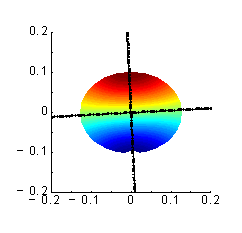
\includegraphics[width=1\linewidth]{./images/SAFE/SAFE_CS_10x8_HTI_45/P_a_7_2kHz-pstool.eps}		
\end{minipage}&
\begin{minipage}{0.22\linewidth}
%	\psfragfig[width=0.22\linewidth,crop=pdfcrop]{./images/SAFE/SAFE_CS_15x10_HTI_45/P_a_3_0kHz}
	
\includegraphics[width=1\linewidth]{./images/SAFE/SAFE_CS_15x10_HTI_45/P_a_3_0kHz-pstool.eps}		
\end{minipage}&
\begin{minipage}{0.22\linewidth}
%	\psfragfig[width=0.22\linewidth,crop=pdfcrop]{./images/SAFE/SAFE_CS_15x10_HTI_45/P_a_7_2kHz}
	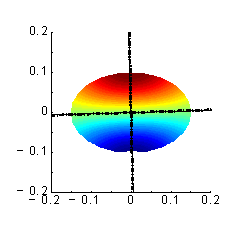
\includegraphics[width=1\linewidth]{./images/SAFE/SAFE_CS_15x10_HTI_45/P_a_7_2kHz-pstool.eps}		
\end{minipage}\\
& \footnotesize НЧФ, 3,03 кГц & \footnotesize ВЧФ, 7,17 кГц & \footnotesize НЧФ, 3,03 кГц & \footnotesize ВЧФ, 7,17 кГц \\ \cline{2-5}
\end{tabular*}
\\
\quad \\
\quad \\
\renewcommand{\arraystretch}{1.0}
\footnotesize
\begin{tabular*}{\textwidth}{@{\extracolsep{\fill} }crccc}
& Результаты обработки		 	&  \textit{1} 	&   \textit{2}	& \textit{3} \\
& Alford rotation: 		& \tikz \draw (0,0) -- (1cm,0); 			& \tikz \draw[dashed] (0,0) -- (1cm,0); 					& \tikz \draw[very thick,dashdotted] (0,0) -- (1cm,0);    			\\
\end{tabular*}
\renewcommand{\arraystretch}{1.0}
%\caption{ \footnotesize Сравнение результатов обработки фильтрованных данных измерений и значений собственных векторов дипольных мод на частоте, соответствующей максимуму энергии в спектре сигнала, в породе Bakken Shale (а) и Cotton Valey Shale (б). Распределение давления (собственный вектор) в сечении скважины показано серым цветом, черные участки соответствуют максимальному и минимальному значениям. НЧФ и ВЧФ соответствуют низкочастотной (НЧФ) и высокочастотной (ВЧФ) фильтрации, применённой к исходным данным.}
\normalsize
\label{fig:comparison_safe_all}
\end{figure}

\end{document}